\documentclass{article}
\usepackage{amsfonts}
\usepackage{graphicx}



\title{
{\large{Univerza v Ljubljani}}\\ 
{\large{Fakulteta za matematiko in fiziko}}\\ 
{\large{Univerzitetni študijski progra Finančna matematika}}\\ 
\vspace{5cm}
{\textbf{Pareto fronte v več dimenzijah}
\vspace{5cm}}
}

\author{Klara Penko, Nejc Jenko}
\date{Januar 2022}


\begin{document}

\begin{titlepage}
    \maketitle
\end{titlepage}

\tableofcontents

\break

\section{Uvod}
V projektni nalogi si bova ogledala Pareto fronte na d-dimenzionalnih množicah. To pomeni, da bova na podani množici poiskala točke, ki so nedominirane. Celotna množica nedominiranih točk je Pareto fronta.  Za opazovane množice točk bova vzela poljubne točke v d-dimenzionalnih kroglah in hiperkockah. Analizirala bova, število točk v Pareto fronti, glede na dimenzijo prostora d. Poleg prve Pareto fronte, bova želela izračunati še drugo, tretjo in tako naprej.


\subsection{Definicija Pareto fronte}
${\rm \textbf{Definicija 1}}$ Naj bo S prostor definiran z množico n dimenzij $\{d_{1},d_{2}\dots,d_{n}\}$ in D podmnožica množice S. Naj bo $p \in D$, podana z $p = (p_{1},p_{2},\dots,p_{n})$, kjer je $p_{i}$ vrednost v dimenziji $d_{i}$. Točka $p \in D$ \textbf{dominira} točko $q \in D$ na podprostoru $S'\subseteq S$, če v vsaki dimenziji $d_{i} \in S'$ velja $p_{i} \le q_{i}$ in v vsaj eni dimenziji $d_{j} \in S'$, $p_{j} < q_{j}$. \\
\underline{\textbf{Pareto fronta}}(oz. 1. Pareto fronta) prostora $S' \subseteq S$ je množica točk $D' \subseteq D,$ ki niso dominirane z nobeno točko v prostoru $S'$. Če točke, ki so v 1. Pareto fornti odstranimo iz mnozice dobimo novo množico. Pareto fronto te množice imenujemo \textbf{2. Pareto fronta}. Ta postopek lahko n-krat ponovimo, da dobimo \textbf{n-to Pareto fronto}.
(Od tu naprej uporablajmo izraz \i{globlja} ko primerjamo dve Pareto fronti na isti množici. Primer: i-ta Pareto fronta je globlja od j-te Pareto fronta, če velja $i > j$.)
\\

${\rm \textbf{Primer Pareto fronte v dveh dimenzijah}}$

\begin{figure}[htbp]
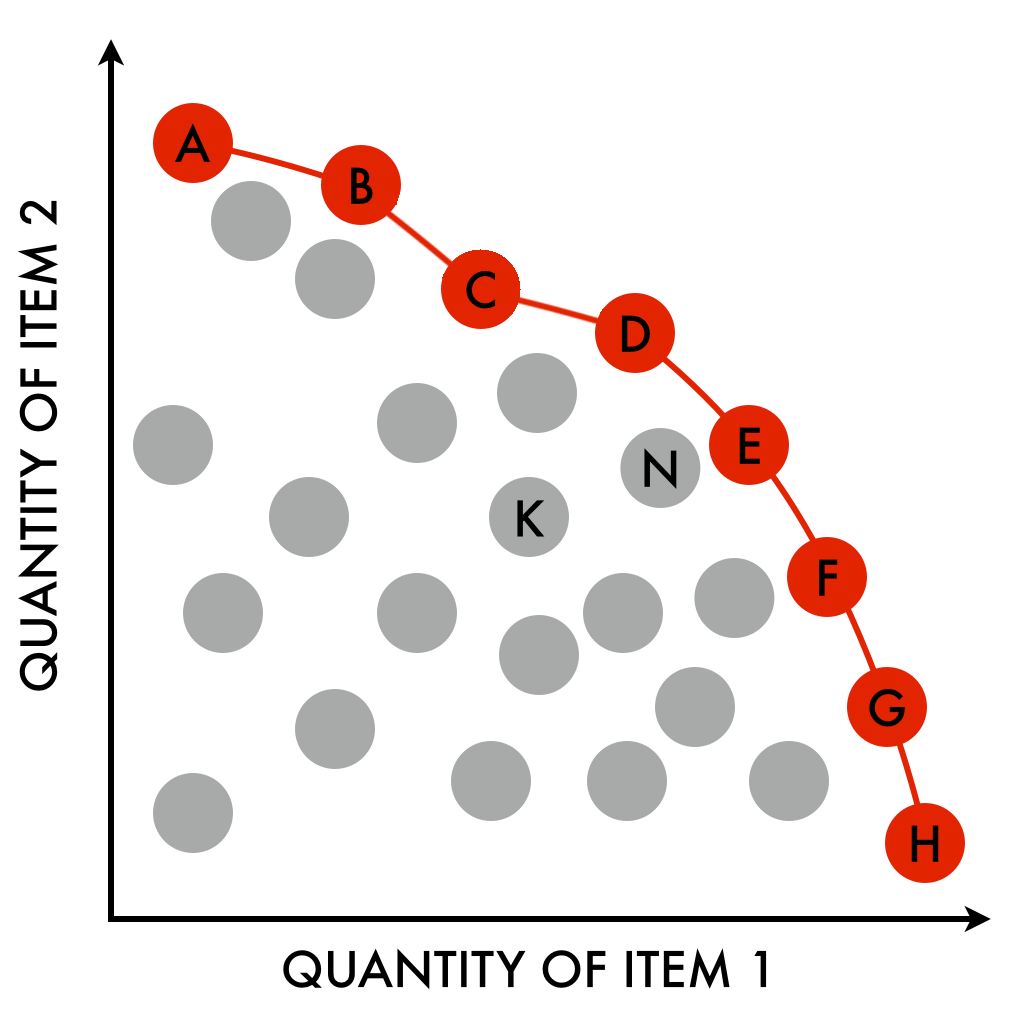
\includegraphics[width=4cm]{Slike/Slika_pareto_fronta.png}
\centering
\end{figure}

\subsection{Hipoteza}
\begin{enumerate}
    \item Predvidevamo, da, če povečujemo dimenzijo, se bo s tem zmanjševalo število točk v globljih Pareto frontah.
    \item Predvidevamo, da bodo imele množice, ki imajo možnost za večje odstopanje v pozitivni smeri vseh oz. več koordinat (npr. kocka napram krogli), v 1. Pareto fronti manjše število točk.
\end{enumerate}

\section{Potek dela}
Za generiranje najinega problema sva uporabila programski jezik Python. Glavni vhodni podatek problema je poljubna množica točk, ki jo lahko ročno izberemo sami, ali pa jo dobimo s pomočjo ene od funkcij, ki sva jih zapisala za generiranje le teh. Zapisala sva funkcijo za izračun Pareto fronte, za katero sva dodatno definirala še eno krajšo funkcijo, kot bomo videli v nadaljevanju. Poleg tega sva zapisala funkciji za generiranje točk v d- dimenzionalni krogli in hiperkocki.

\subsection{Funkcije za izračun Pareto fronte}

Glavna funkcija najine projektne naloge je funkcija \textbf{izracun\_pareto\_fronte}, ki sprejme množico točki in vrne pareto fronto, ter množico dominiranih točk. Vmes pa se v kodi te funkcije pojavi še funkcija \textbf{dominira}. Koda obeh je zapisana spodaj.

\begin{verbatim}

def dominira(a, b):
    return sum([a[x] >= b[x] for x in range(len(b))]) == len(b)
\end{verbatim}

Ta funkcija sprejme dve točki(poljubne iste dimenzije) in vrne \textbf{True}, če točka a dominira točko b. Funkcijo \textbf{dominira} uporabimo v naslednji kodi.

\begin{verbatim}

def izracun_pareto_fronte(mnozica): 
    pareto_fronta = set()
    dominirane_tocke = set()

    while len(mnozica) != 0:
        kandidat = list(mnozica)[0] 
        mnozica.remove(kandidat)
        i = 0
        ni_dominirana = True 

        while i < len(mnozica):
            tocka = list(mnozica)[i]
            if dominira(kandidat, tocka): 
                mnozica.remove(tocka)
                dominirane_tocke.add(tuple(tocka))
            elif dominira(tocka, kandidat):
                dominirane_tocke.add(tuple(kandidat))
                ni_dominirana = False
                break
            else:
                i += 1

        if ni_dominirana:   
            pareto_fronta.add(tuple(kandidat))
        
    return pareto_fronta, dominirane_tocke

  
\end{verbatim}

V zgornji fuknciji najprej določimo prazne množice za iskano množico Pareto fronta in iskano množico dominiranih točk. Najprej si iz množice, ki jo podamo funkciji izberemo prvega kandidata in ga odstranimi iz prvotne množice. Za tega preverimo ali ta dominira točke, ki so še ostale v množici oziroma če katera od točk iz množice dominira izbranega kandidata. V primeru, da kandidat dominira točko, jo dodamo v množico, ki nam bo vrnila dominirane točke.  Ta postopek ponavljamo dokler, ne pregledamo vseh točk iz podane množice (tj. podana množica je prazna). Tako nam zapisana funkcija vrne iskano Pareto fronto, ter množico dominiranih točk.


\subsection{Funkcija za izračun n pareto front}
Poleg računanja prve Pareto fronte, sva se lotila pisanja kode za funkcijo, ki bo vrnila n Pareto front. Spodnja funkcija, kot argument sprejme poljubno množico točk, ter število n. S številom n povemo koliko Pareto front, bi želeli izračunati. Pareto fronte, tukaj izračunamo rekurzivno s pomočjo zgoraj definirane fukncije izracun\_pareto\_fronte. Množico zmanjšujemo, dokler ne pridemo do željene Pareto fronte oziroma dokler ne izpraznimo podane možice točk.

\begin{verbatim}
def izracun_n_pareto_front(mnozica, n): 
    if len(mnozica) == 0:   
        return set()
    elif n < 1:
        return set()    
    else:
        pareto, dom = izracun_pareto_fronte(mnozica)
        print(len(pareto))  
        return pareto, izracun_n_pareto_front(dom, n-1)
\end{verbatim}

\subsection{Funkcija za generiranje točk na d-dimenzionalni enotski krogli}
Funkciji \textbf{random\_krogla} podamo število točk, ki jih želimo zgenerirati in dimenzijo prostora, dodatno lahko spremenimo tudi parameter radij, če bi gledali neenotske krogle (tj. radij krogle različen od 1). V kodi najprej zgeneriramo naključni vektor dimenzije d in ga normiramo. Dobljeni vektor pomnožimo z naključno vrednostjo med 0 in 1, da dobimo točko v notranjosti d dimenzionalne krogle. Na ta način zgeneriramo toliko točk, kot smo podali z atributom stevilo\_tock.
\begin{verbatim}
def random_krogla(stevilo_tock, d, radij=1):
    mnozica_tock = set()
    for i in range(stevilo_tock):    
        rand_smer = random.uniform(low=-1, high=1, size=d) 
        rand_smer /= linalg.norm(rand_smer, axis=0) 
        rand_dolzina = random.uniform(low=0, high=1) 
        tocka = tuple(radij * (rand_smer * rand_dolzina)) 
        mnozica_tock.add(tocka)
    return mnozica_tock
\end{verbatim}


\subsection{Funkcija za generiranje točk na hiperkocki s stranico a}
Podobno, kot smo zgenerirali točke znotraj enotske d-dimenzionalne krogle, zdaj zgeneriramo točke znotraj hiperkocke. Funkciji podamo število točk, dimenzijo prostori in stranico hiperkocke a. Če stranice ne podamo, funkcija privzeto zgenerira točke v enotski hiperkocki. V kodi zgeneriramo naključen vektor velikosti d, z vrednostmi med 0 in a, kar nam predstavlja eno točko. In tako zgeneriramo toliko točk kot smo podali.
\begin{verbatim}
def random_kocka(stevilo_tock,d,a=1): 
    mnozica_tock = set()
    for i in range(stevilo_tock):
        rand_smer = random.uniform(low=0, high=a, size=d)
        tocka = tuple(rand_smer)
        mnozica_tock.add(tocka)
    return mnozica_tock
\end{verbatim}





\section{Eksperimentalni Del}

Ko imamo napisane funkcije za generiranje podatkov in njihovo obdelavo, lahko začnemo z eksperimentalnim delom. Naše eksperimente bomo ločili na dva dela. V prvem delu si bomo pogledali vpliv višanja dimenzije prostora. V drugem delu pa bomo v isti dimenziji primerjali rezultate, če testne točke generiramo na različnih območjih (enotska krogla in enotska kocka). Vsi konkretni podatki so dostopni v priloženem .xlsx dokumentu.

\subsection{Prvi Del - Vpliv dimenzije}
V prvem delu bomo za svoje podatke generirali 2, 3, 4 in 5 dimenzionalne krogle in primerjali število točk v prvih petih Pareto forntah. Za vsako dimenzijo bomo opazovali množice po 50, 100 in 200 točk. Za vsako od teh kombinacij bomo poskus ponovili desetkrat. V spodnjih grafih so prikazana povprečna števila točk v vsaki Pareto fronti.

\break
\begin{figure}[htbp]
    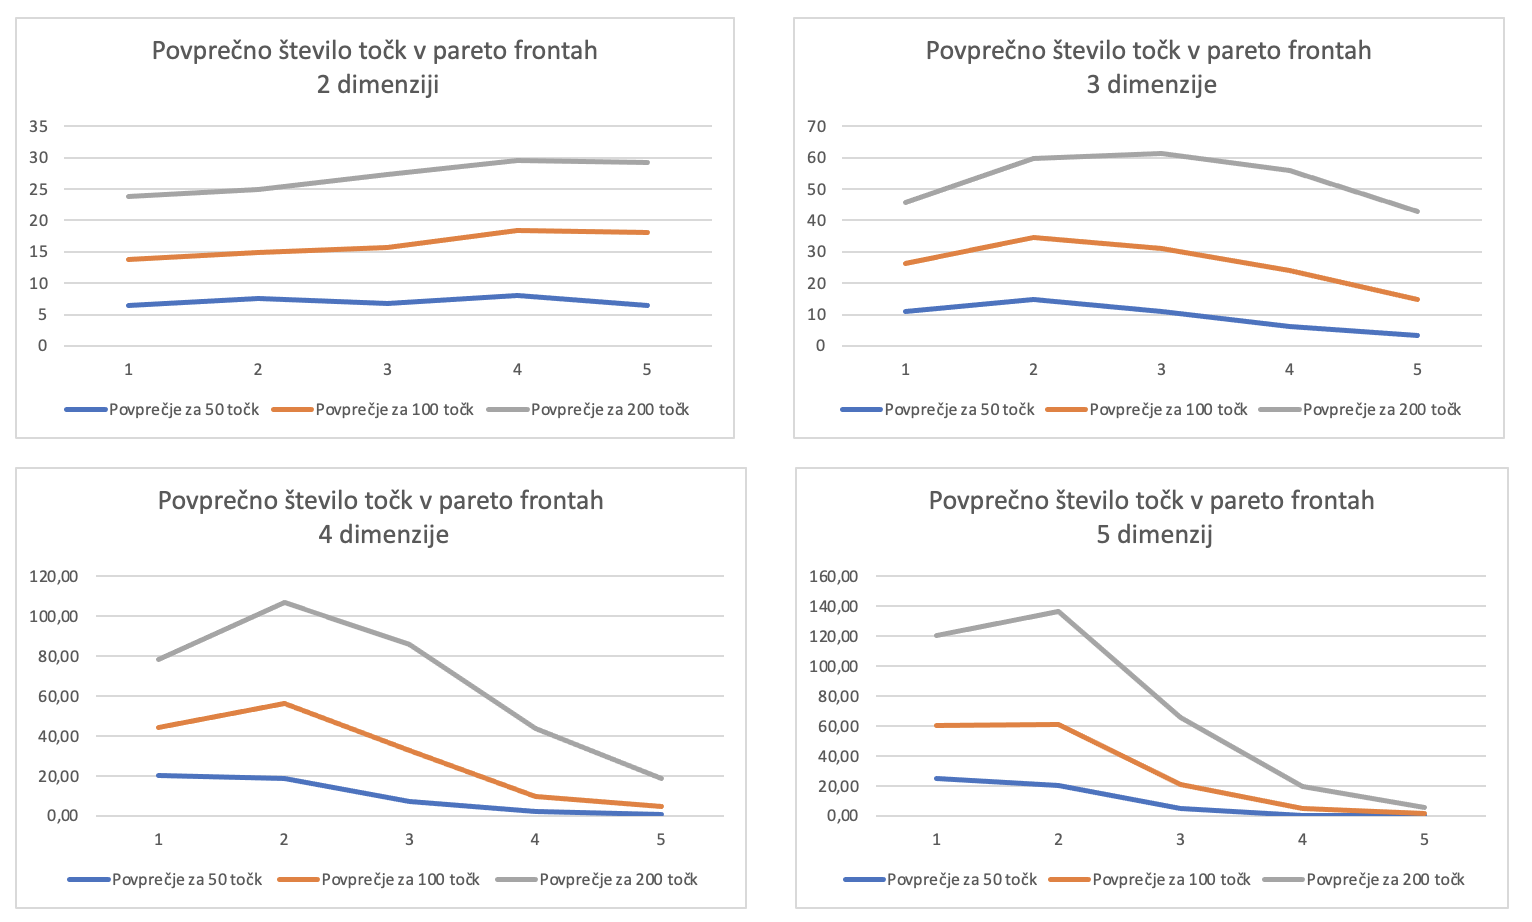
\includegraphics[width=130mm]{Slike/Graf1.png}
\centering
\end{figure}

Kot lahko vidimo iz zgornjih grafov, se z višanjem dimencije delež točk v manj globokih Pareto forntah povečuje. Pri dvodimenzionalni krogli imamo v prvih petih Pareto frontah približno enako točk. V naših poskusih jih je v 1. Pareto fronti celo manj točk kot v 5. Pareto fronti. Pričakujemo lahko, da bi z večanjem števila poskusov, ne glede na število generiranih točk, vse krivulje na grafu postajale vedno bolj linearne. Pri povečanju dimenzije na 3 že opazimo trend, da maksimalno število točk dobimo v 2. oz 3. Pareto fronti. To predvidevamo, da je posledica tega, da v 1. Pareto fronti zajamemo najbolj izstopajočje točke, ki dominirajo velik delež ostalih točk. Pri 2. in 3. pareto fronti pa opazujemo že bolj "zglajeno" množico, zato v pareto fronti dobimo več točk. V treh dimenzijah začenjamo opažati tudi vpliv števila generiranih točk. Z več generiranimi točkami se spremembe kažejo bolj intenzivno. Ko dimenzijo povečamo na 4 ali 5 se nam pokaže očiten maksimum števila točk v 2. Pareto fronti. v teh primerih skoraj vse točke množice zajamemo že v prvih treh Pareto frontah. Do tega po našem mnenju pride, ker imamo v več dimenzijah več kriterijov, po katerih mora biti točka dominirana, da izpade iz Pareto fronte. \\
\texttt{Opazimo lahko, da eksperiment potrjuje našo prvo hipotezo.}

\subsection{Drugi del - Vpliv oblike množice}
V drugem delu si bomo pogledali primerjavo v številu točk v Pareto frontah, če naše testne točke generiramo v enotski krogli ali pa v hiperkocki s stranico dolžine 1. Pri eksperimentu bomo za vsak primer izvedli 20 poskusov. Tokrat bomo poskuse delali z 500 točkami in v 5 dimenzijah. 5 dimenzij smo izbrali, ker se v tem primeru že bolje vidi upad števila točk v globjih Pareto frontah. Ker pa je ta upad tako velik, smo število generiranih točk povečali na 500. S tem smo želeli preprečiti, da bi že v manj kot 5 Pareto frontah zajeli vse točke iz naše testne množice.

\begin{figure}[htbp]
    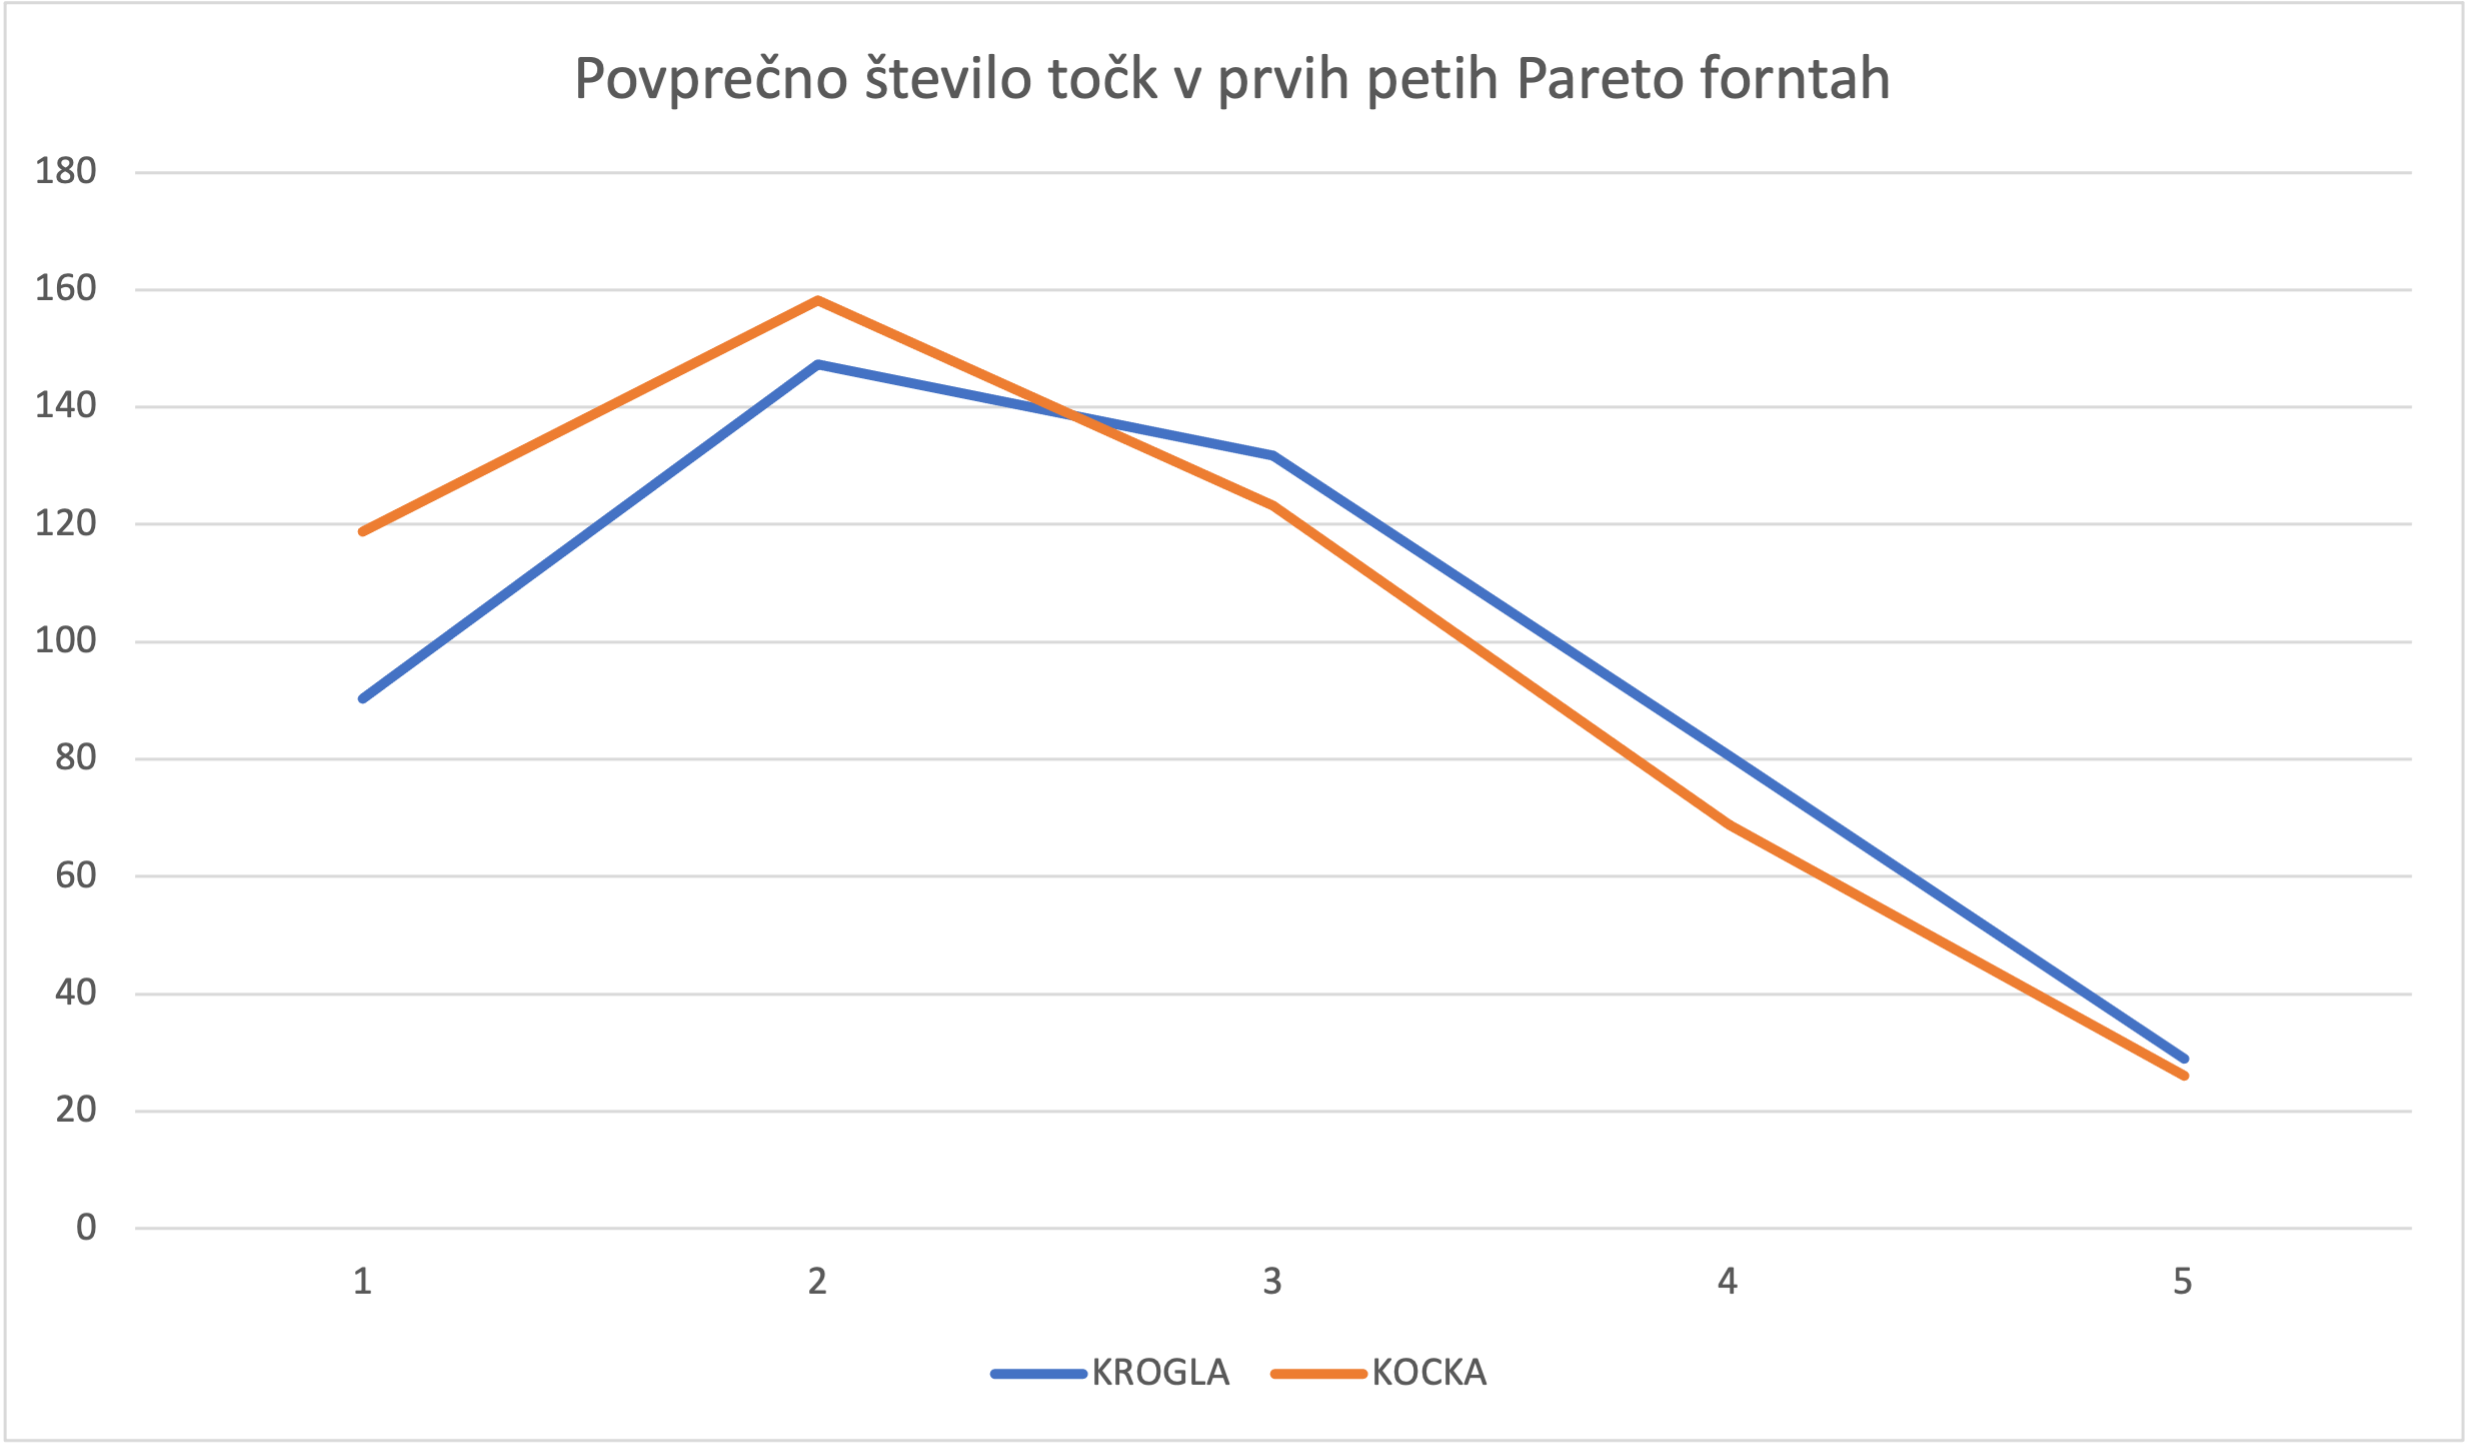
\includegraphics[width=130mm]{Slike/Graf2.png}
\centering
\end{figure}

Kot lahko vidimo iz zgornjega grafa, do največjega odstopanja pride v 1. Pareto fronti, kjer je pri množici generirani v hiperkocki v povprečju skoraj 30 točk več, kot pri množici generirani v krogli. To je v nasprotju z našimi pričakovanji. Pričakovali smo, da bodo točke, ki bodo v kotu hiperkocke z največjimi vrednostmi v vseh koordinatah dominirale velik del množice in zato zmanjšale število točk v 1. Pareto fronti. \\
Prav tako je tudi pri pregledu 2. Pareto fronte še vedno več točk pri hiperkocki. Trend se obrne šele v 3. Pareto fronti, od koder obe krivulji enakomerno padata. \\
Če privzamemo, da je prišlo do odstopanja zaradi naključnih podatkov, lahko rečemo, da oblika množice ni imela velikega vpliva na število točk v Pareto frontah.
\texttt{Opazimo, da se eksperiment ne sklada z našo drugo hipotezo.}

\subsection{Časovna zahtevnost}
Naj bo $n$ število generiranih točk, $d$ dimenzija prostora in $m$ globina Pareto front. 
\begin{itemize}
    \item Za generiranje točk v krogli uporabljamo \texttt{for} zanko z $n$ ponovitvami. V vsaki ponovitvi opravimo $d$ korakov za generiranje vektorja, $2d + 1$ korakov za računanje norme, $d$ korakov za deljenje vektorja z normo, 1 korak za generiranje dolžine, $2d$ korakov za množnje vektorja z dolžino in radijem in  1 korak za dodajanje točke v množico. \\
    Pri generiranju točk v hiperkocki prav tako uporabimo $n$ ponovitev zanke. V tem primeru pa v vsaki ponovitvi izvedemo le $d$ korakov za generiranje točke in 1 korak da točko dodamo v množico. \\
    Torej, pri generiranju podatkov v obeh primerih za izvedbo funkcije potrebujemo $O(nd)$ korakov. 
    \item Pri funkciji za računanje Pareto fronte uporabimo 2 gnezdeni \texttt{while} funkciji. Iz ustavitvenih pogojev lahko ugotovimo, da bo maksimalno število ponovitev prve zanke $n$, maksimalno število ponovitev druge zanke pa $n-1$. V drugi zanki nato dvakrat uporabimo funkcijo \texttt{dominira}, za katero potrebujemo $d$ korakov. Skupno število korakov je torej:
    $$
        n (4 + (n-1) (1 + d + d + 1) + 1 + 1) + 1 = 
        2n^2d + 2n^2 - 2nd + 4n + 1.
    $$
    V skupnem lahko velikostni razred označimo z $O(n^2d)$. V realnosti je število korakov lahko precej manjše, saj lahko v vsaki ponovitvi odstranimo več kot 1 točko.
    \item Pri računanju m-te Pareto fronte $m$-krat rekurzivno uporabimo funkcijo. Torej je velikostni razred časovne zahtevnosti $O(n^2dm)$. V realnosti je tudi tu zahtevnost manjša, saj v vsaki ponovitvi rekurzije delamo s precej manjšo množico točk.
\end{itemize}
 
\section{Zaključek}
Pareto fronta je podmnožica vseh točk za katere velja, da niso dominirane s strani nobene druge točke iz začetne množice. Iz naše analize podatkov smo lahko dognali močno korelacijo med dimenzijo prostora, kjer izbiramo točke in številom točk v 1., 2., 3., ... Pareto fronti. Z večanjem dimenzije se je povečevalo tudi število točk v prvih treh Pareto frontah, kar je podprlo našo prvo hipotezo. Opazili smo tudi, da oblika množice, v katerih smo generirali naše testne točke, ni imela pretiranega vpliva na število točk v Pareto frontah. Ta opazka je nasprotovala naši drugi hipotezi.


\end{document}